%%%%%%%%%%%%%%%%%%%%%%%%%%%%%%%%%%%%%%%%%%%%%%%%%%%%%%%%%%%%%%%%%%%%%%%%%%%%%%%%%%%%%%%%
%
%   Context of the Project                   
%
%%
%%%%%%%%%%%%%%%%%%%%%%%%%%%%%%%%%%%%%%%%%%%%%%%%%%%%%%%%%%%%%%%%%%%%%%%%%%%%%%%%%%%%%%
\section{Introduction}

\subsection{Context}

%Dans un monde de plus en plus connecté et soucieux de l’environnement, nos maisons se transforment en habitats intelligents, et permettent notamment une meilleure gestion des dépenses énergétiques au quotidien. Ces dernières années, de nombreux systèmes de domotique assurant la gestion des équipements (portails, volets, lumières) sont arrivés sur le marché. Néanmoins, très peu de ces systèmes permettent le suivi détaillé et le pilotage énergétique de l’ensemble des équipements au sein de l’habitat. Période de crise et diminution du pouvoir d’achat poussent les Français à réaliser des économies dans tous les domaines. Selon l’ADEME (Agence de l’environnement et de la maîtrise de l’énergie), la facture moyenne (toutes énergies confondues) s’est élevée en 2012 à 1 403 euros par ménage, contre 1 239 euros en 2007. Aujourd’hui, 80\% des ménages cherchent à réduire leur consommation d’énergie, notamment via des comportements plus économes en terme d’éclairage et de chauffage. Un nouveau secteur est en train de naître, les smart energy boxes. Certains fabricants du domaine énergétique tels que Legrand ou Schneider Electric proposent déjà des solutions comme les premiers compteurs électriques connectés. Le projet Ecobox s’inscrit dans une démarche de meilleure gestion de l’énergie par un pilotage autonome et automatisée de l’habitat.

\subsection{Smart EcoBox Description}
% Quel est le but de la box ?
% 
% déroulement du process : recevoir trame, décoder, inserer dans db. detection des états des appareils. affichage des infos sur le client.
%
% pourquoi avoir choisi Raspberry Pi ?
%   box doit être petite (cad pas un gros pc etc..)
%   peu cher -> correspond au souhait du client d'avoir une box abordable
%   comme ça a peu de ressources, si ça passe dessus peu importe les ressources dispo dans le future


The \textbf{Smart EcoBox} project is aimed to help people manage their energy consumption and therefore enabled a reduction of their energy bills. 

%La gestion des équipements de la maison par l’intermédiaire de terminaux tels que tablettes ou téléphones permettra de simplifier la vie de l’utilisateur au quotidien.

\begin{figure}[H]
\centering
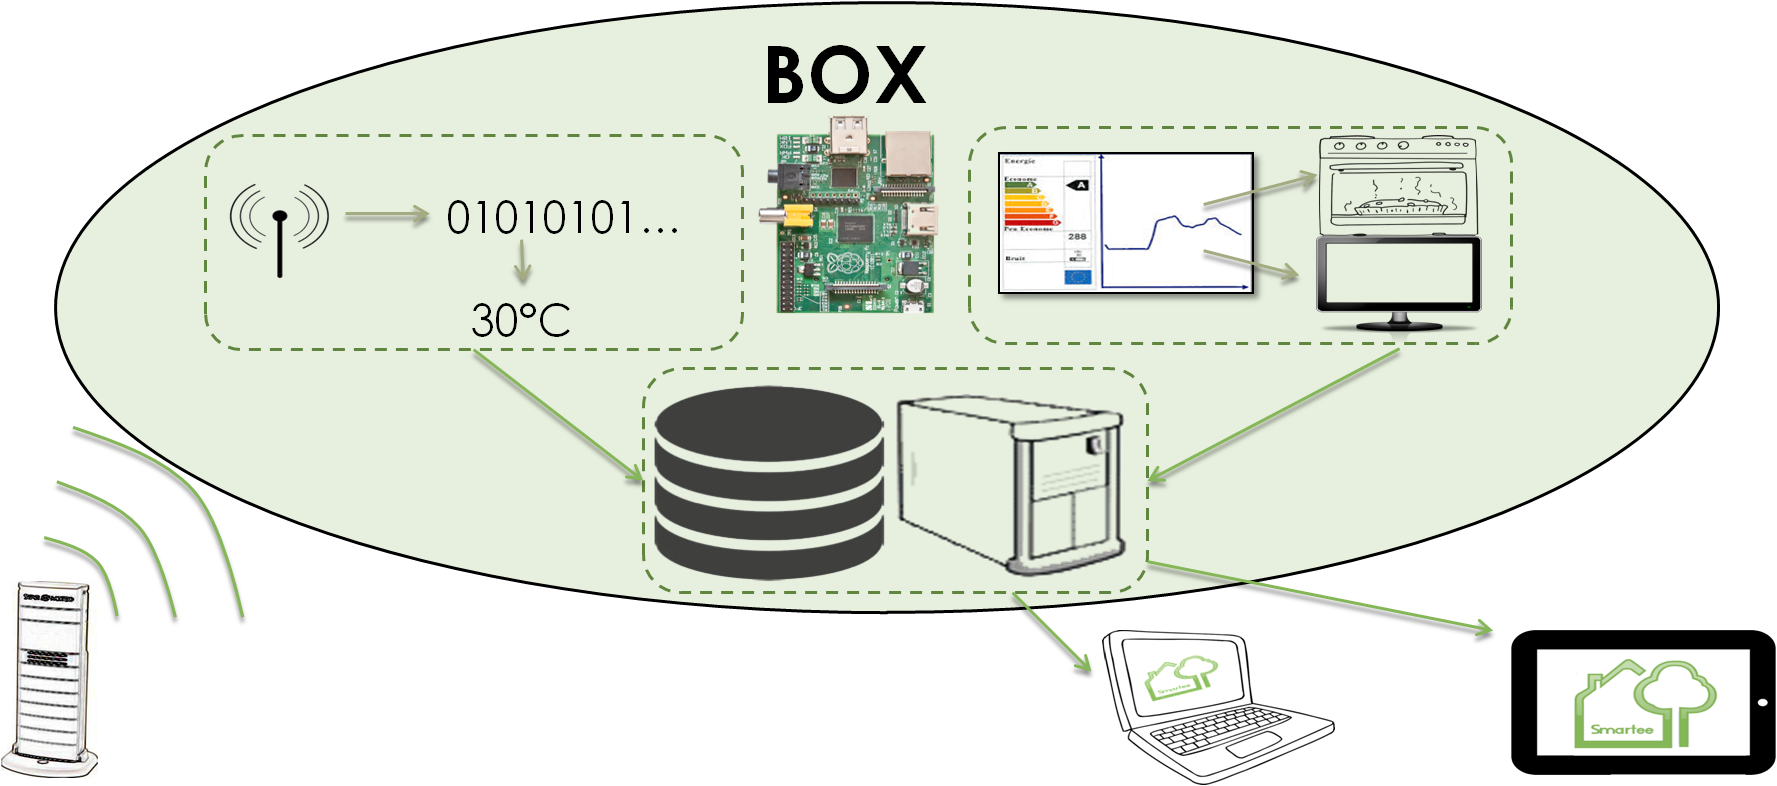
\includegraphics[scale=0.4]{img/box.png}
\caption{Smart Eco Box Description}
\label{fig:boxDescription}
\end{figure}


